%!TEX root = oral.tex

\section{Routing problem for autonomous ride-share}

	\begin{frame}
	\textbf{Paper 2: Robotic load balancing for mobility-on-demand systems}
	\begin{itemize}
		\item Marco Pavone \\
		\textit{Stanford University}
		\item Stephen L. Smith \\
		\textit{University of Waterloo}
		\item Emilio Frazzoli \\
		\textit{Massachusetts Institute of Technology}
		\item Daniela Rus \\
		\textit{Massachusetts Institute of Technology}
	\end{itemize}
	\end{frame}

    \begin{frame}{Fluid model}
        \begin{figure}
            \centering
            {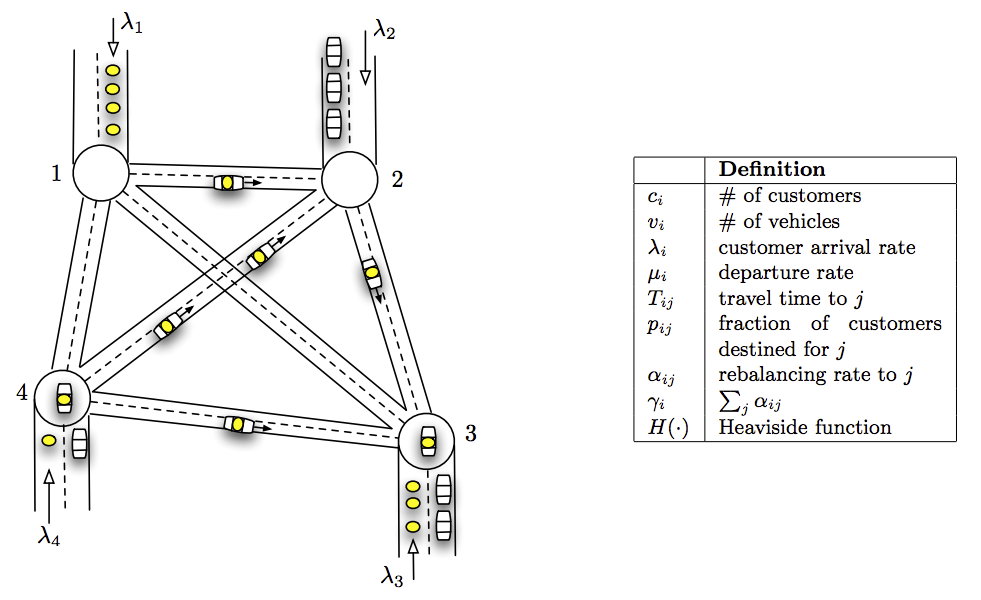
\includegraphics[scale=0.28]{plots/fluid_model.png}}
            \caption{Fluid model for autonomous cars\footcite{pavone2012robotic}.}
        \end{figure}
    \end{frame}

    \begin{frame}{Existence of equilibrium}
    Let $\mathcal{A}$ be set of assignments of $\alpha$ that verify equation
    \begin{equation*}
    \sum_{j \neq i}\alpha_{ij} + \lambda_i = \sum_{j \neq i}\alpha_{ji} + \sum_{j \neq i}\lambda_j p_{ji}
    \end{equation*}
    for each $i \in \mathcal{S}$, 
    \pause
    and let
    \begin{equation*}
    V_{\alpha} = \sum_{ij} T_{ij}(p_{ij} \lambda_i + \alpha_{ij})
    \end{equation*}
    \pause
    then,
    \begin{enumerate}
        \item if $V > V_\alpha$, then there exists an equilibrium assignment of $\alpha$.
        \item if $V \leq V_\alpha$, then no equilibrium exists.
    \end{enumerate}
    \pause
    \alert{$V^* = \min_{\alpha \in \mathcal{A}}V_{\alpha}$ is minimum number of vehicles required for existence of equilibrium.}
    \end{frame}

    \begin{frame}{Optimal Re-balancing}
    Minimize
    \begin{equation*}
    \sum_{ij} T_{ij}\alpha_{ij}
    \end{equation*}
    subject to
    \begin{align*}
        \sum_{j \neq i}\alpha_{ij} + \lambda_i = \sum_{j \neq i}\alpha_{ji} + \sum_{j \neq i}\lambda_j p_{ji} && \forall i \in \mathcal{S} \\
        \alpha_{ij} \geq 0 && \forall{i,j} \in \mathcal{S}
    \end{align*}
    \pause
    \only<2>{\alert{Minimizing $\sum_{ij} T_{ij}\alpha_{ij}$ also leads to minimizing $V_\alpha$ (total vehicle utilization).}}
    \pause
    If we impose triangle inequality on travel times $T_{ij}$, then stations can be divided into those with a \textit{surplus} ($S$) and those with a \textit{deficit} ($D$), where $S = \big\{i \in \mathcal{S} | \lambda_i < \sum_j \lambda_j p_{ji}\big\}$ and $D = \mathcal{S} \setminus S$.
    \end{frame}

    \begin{frame}{Continuous bipartite matching}
    Minimize
    \begin{equation*}
    \sum_{i \in S, j \in D} T_{ij}\alpha_{ij}
    \end{equation*}
    subject to
    \begin{align*}
        \sum_{j \in D}\alpha_{ij} = - \lambda_i + \sum_{j \neq i}\lambda_j p_{ji} && \forall i \in S \\
        \sum_{i \in S}\alpha_{ij} = \lambda_j - \sum_{i \neq j}\lambda_i p_{ij} && \forall j \in D \\
        \alpha_{ij} \geq 0 && \forall{i,j} \in \mathcal{S}
    \end{align*}
    \pause
    \begin{itemize}
        \item Fewer variables and fewer constraints.
        \pause
        \item Linear Program.
    \end{itemize}
    \end{frame}

    \begin{frame}{Summary}
    	\textbf{Positives:}
    	\begin{itemize}
    		\item Fluid models make it easy to analyze system dynamics.
    		\item Allows us to study stability of equilibrium.
    	\end{itemize}
    		\vspace{0.1in}
    		\pause
    	\textbf{Concerns:}
    	\begin{itemize}
    		\item \alert{Only for the case of constant flow rates.}
    		\item \alert{Susceptible to perturbations in $p_{ij}$.}
    	\end{itemize}
    \end{frame}